\chapter{实现细节与结果分析}\label{chap:experiment}

\section{ADMM动力学解算}\label{sec:experiment-admm}

尽管前文已经给出了用于流固耦合的具体方法(算法\ref{alg:ipc-fluid-final}),但作为本设计的另一重要部分,本节将详细阐述基于ADMM方法实现的动力学求解算法,即DynamicLocalStep和DynamicGlobalStep的具体细节。

在\ref{sec:admm}中已经详细阐述了弹簧质点PD的算法(Local/Global),并分析了其与ADMM算法的联系。在本文具体的实现中,相较于PD算法,我们修改了$\rho = 1$。此时Local Step即为DynamicLocalStep,Global Step即为DynamicGlobalStep。

不同于原先PD的算法,我们在弹簧质点模型中使用了Consensus ADMM算法,类似于Jacobi迭代,是一个无矩阵的方法,非常利于并行计算实现。其修改了Global Step,相较于求解矩阵
\begin{equation}
  \mathbf A \mathbf x = \mathbf b
\end{equation}
其使用了单步的Jacobi迭代近似该方程的解:
\begin{equation}
 \left(\frac{m_i}{h^2} + \sum_{(i, j) \in \mathcal C} k_{ij}\right) \mathbf x^{(k+1)}_i = \frac{m_i}{h^2} \mathbf y_i + 
\sum_{(i, j)\in \mathcal C} k_{ij} (\mathbf x^{(k)}_j + \mathbf d) 
\end{equation}
该方法相较于原先的PD方法有较大的性能提升,如\ref{tab:ms}。
\begin{table}
  \centering
  \begin{tabular}{l|cc}
    模型尺寸& Consensus ADMM & PD\\
    \hline
    10$\times$10 & 1.4ms & 2.7ms \\
    100$\times$100 & 22ms & 75ms \\
    200$\times$200 & 80ms & 353ms
  \end{tabular}
  \caption{Consensus ADMM与PD对比:在不同场景下,Consensus ADMM相较于PD有2~5倍的性能提升。}\label{tab:mass-spring-benchmark}
\end{table}

\begin{figure}[hbt]
  \centering
  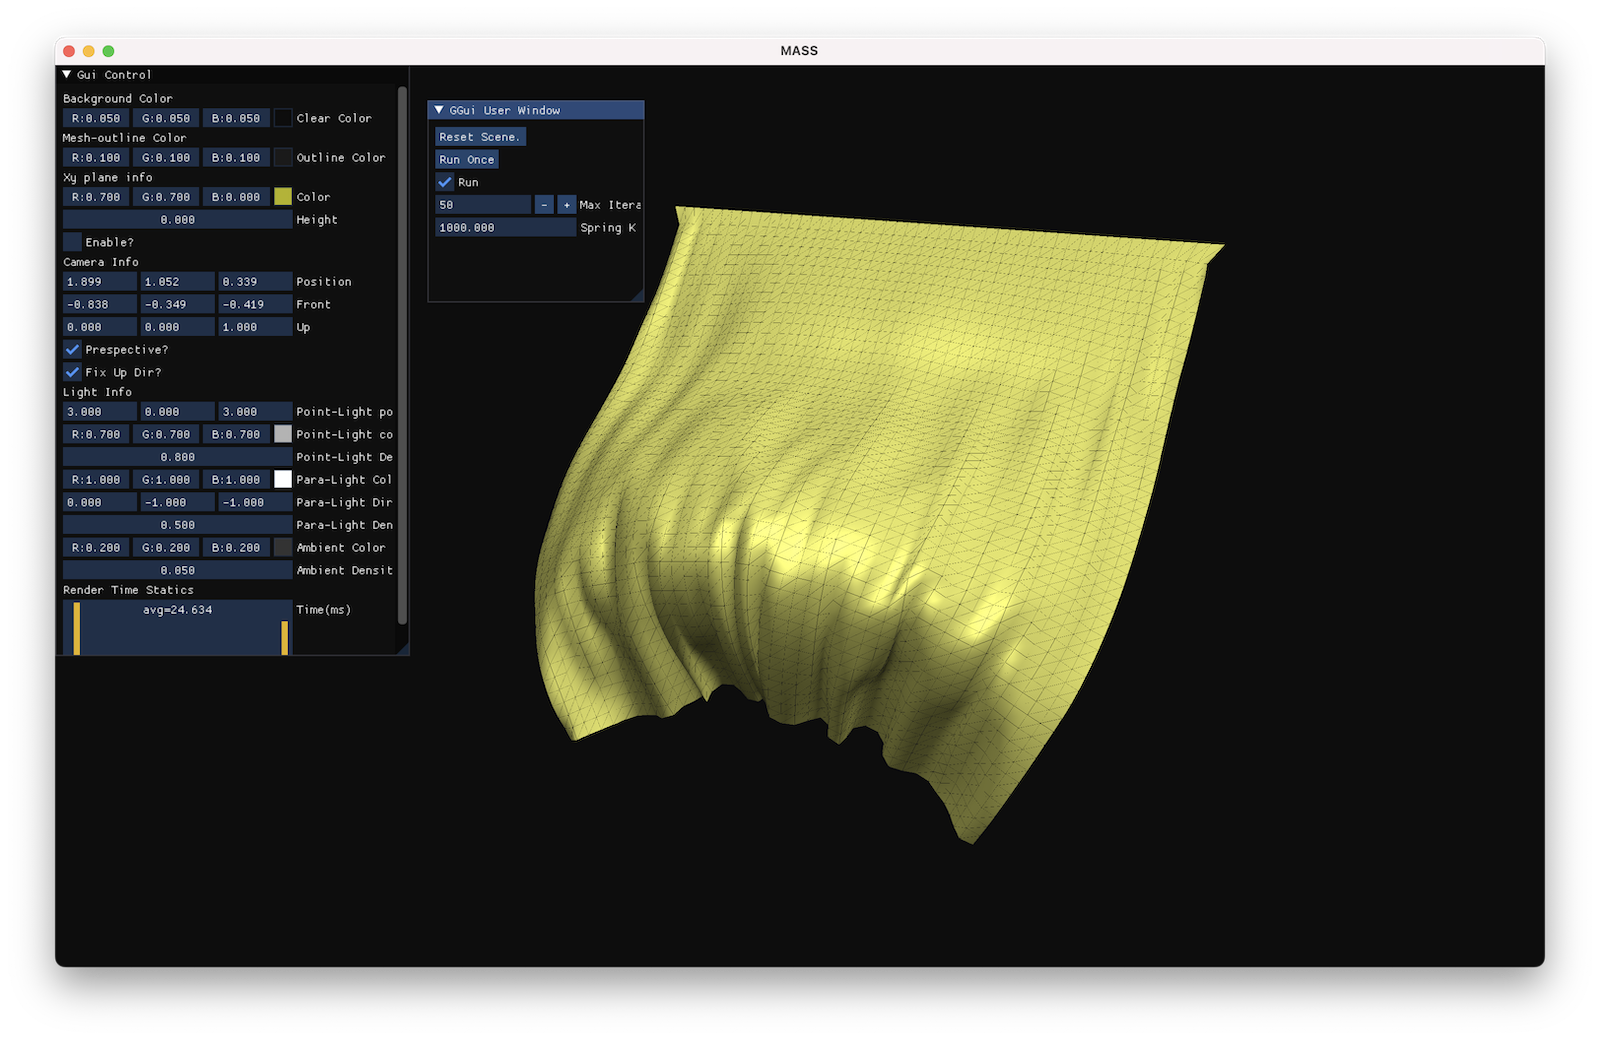
\includegraphics[width=0.8\linewidth]{img/mass-sp-result-norend.png}
  \caption{弹簧质点模型仿真结果}
\end{figure}

对于有限元法,DynamicLocalStep是对于每一个四面体$\mathbf D \mathbf x = [\mathbf x_2 - \mathbf x_{1},\mathbf x_3 - \mathbf x_{1}, \mathbf x_4 - \mathbf x_1]$,求解:
\begin{equation}
  \argmin{\mathbf Z} \frac{\rho}{2}\| \mathbf{Dx} - \mathbf{Z} \|_2^2 + u^{T} (\mathbf{Dx} - \mathbf{Z}) + \Phi(\mathbf Z)
\end{equation}
但考虑到\ref{eq:deformation-grad-compute},$\Phi$的计算依赖于形变梯度矩阵$\mathbf F = \mathbf Z\mathbf X_{rest}^{-1}$,为了减少计算 $\mathbf F$ 的开销,在这里存储形变梯度矩阵作为ADMM的松弛变量,而非直接为$\mathbf Z$,此时的ADMM的等式约束求解被转化为:
\begin{equation}
  \mathbf{Dx} - \mathbf{FX}_{rest}^{-1} = \mathbf 0
\end{equation}

其优点在于,在Local Step的迭代中,$\Phi(\mathbf F)$的实现是相对简单的,且不需要复杂的从$\mathbf X_{rest}$恢复对$\mathbf {Dx}$的操作。对于$\Phi$及其导数的实现,使用了基于Smith不变量的方法实现,而非传统的Cauchy不变量。尽管其只适用于一些简单模型,但其在实现上更为简单,计算更加高效,在图形学中较常用。

用于动力学求解的一个场景如图\ref{fig:hybrid-admm-result}所示。其性能能基本达到实时要求。(3\~10fps,其中有限元模型有400个节点,1384个四面体元, NeoHookean)

\begin{figure}[hbt]
  \centering
  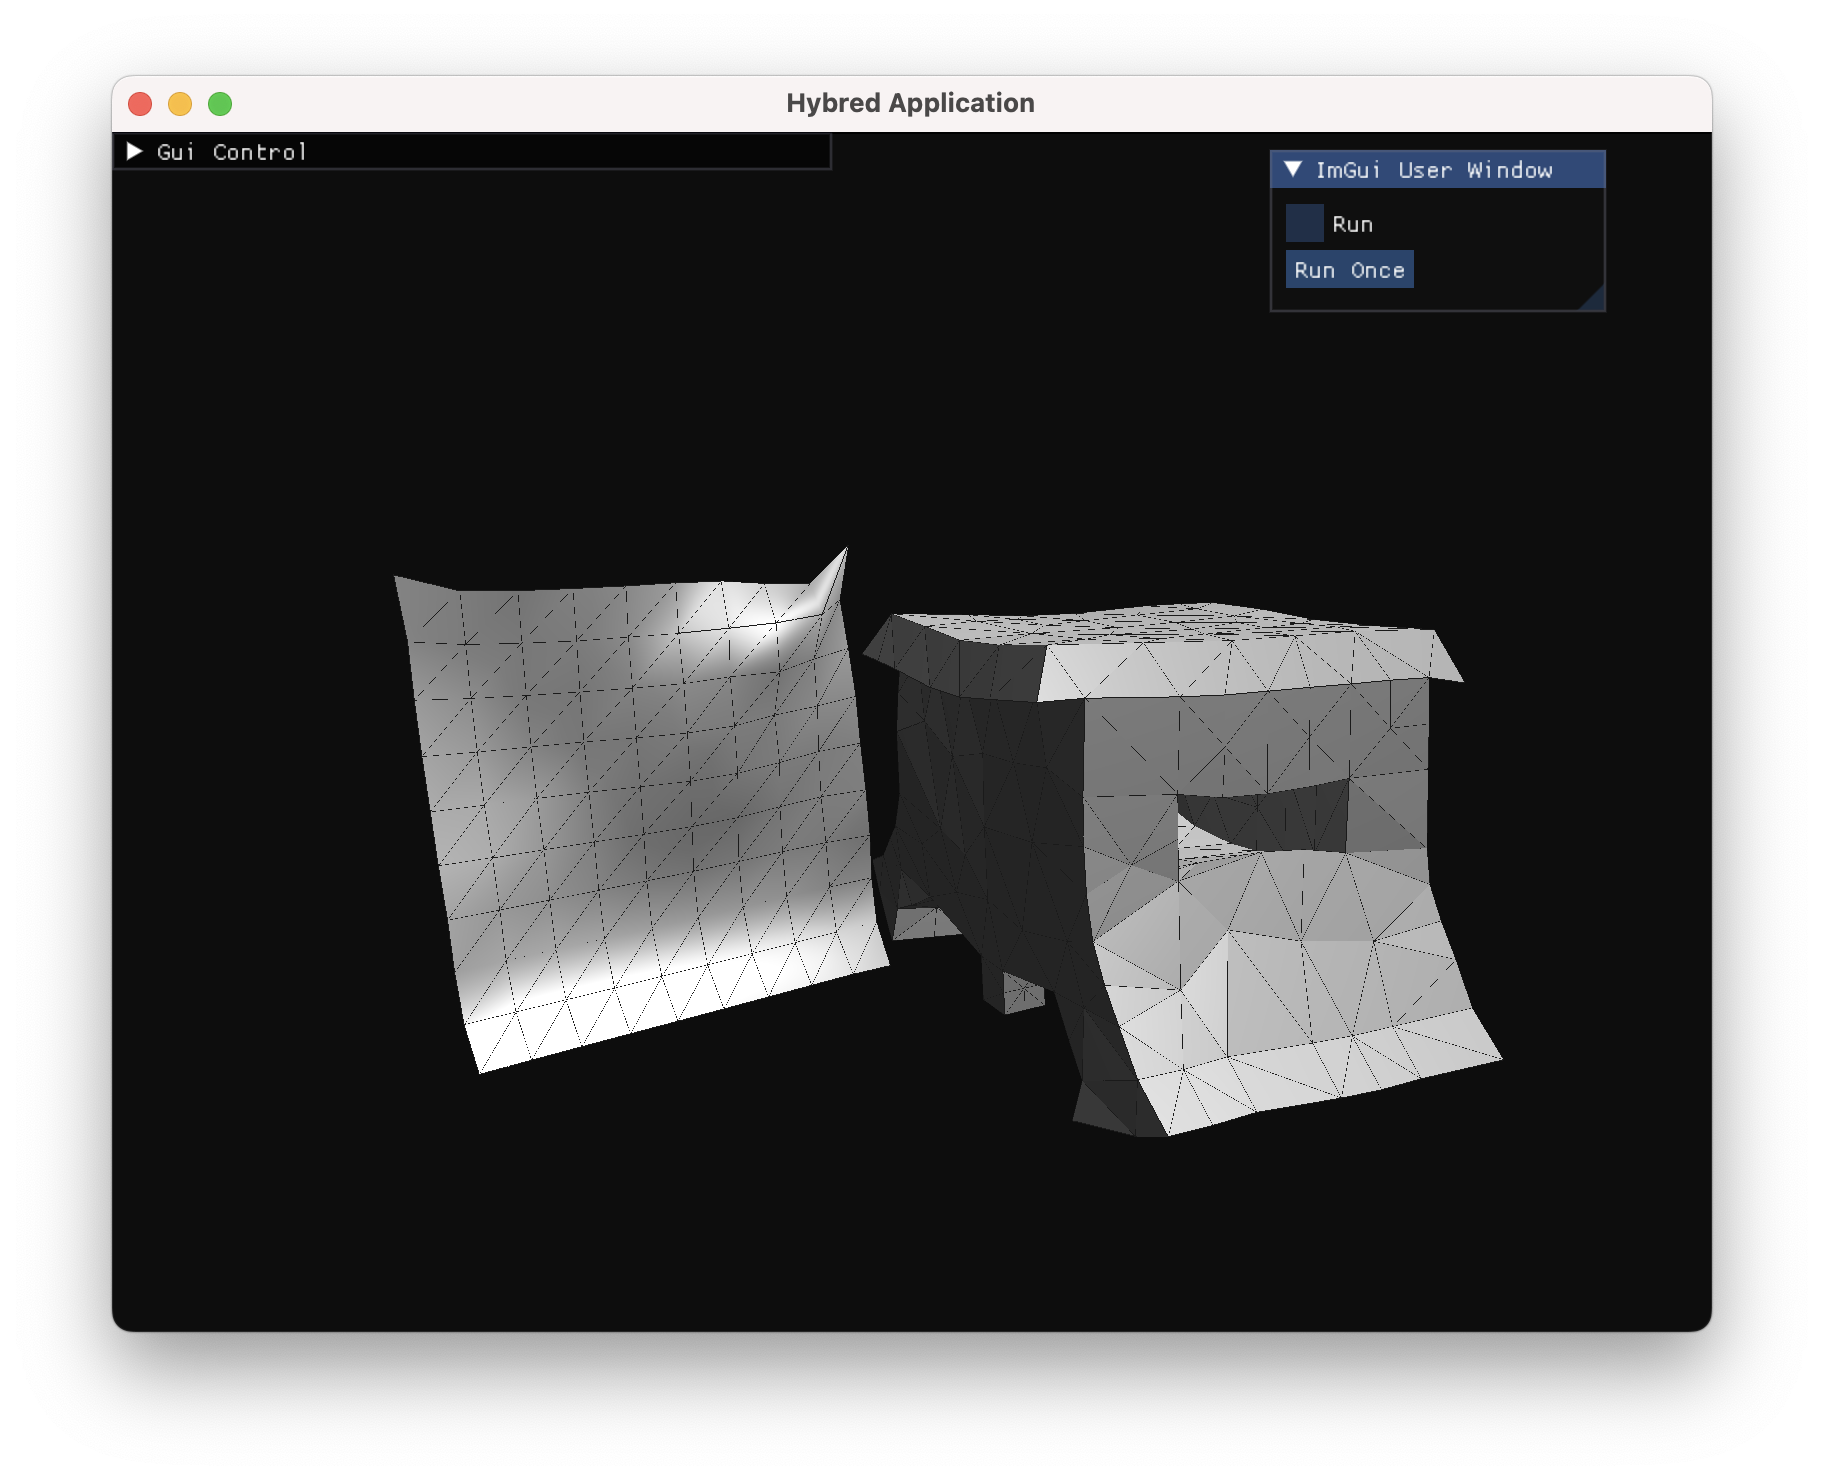
\includegraphics[width=0.75\linewidth]{img/hybrid-admm.png}
  \caption{有限元法、弹簧质点模型统一场景仿真结果}\label{fig:hybrid-admm-result}
\end{figure}


\section{两阶段碰撞检测算法}\label{sec:collid-detect}

尽管ADMM-IPC算法已经完善,但通过分析解算占用的时间可以看到,CCD计算,即碰撞相关计算占据的时间相较其他步骤都高,因此在本章也将详细阐述本文实现的碰撞检测算法。通常而言,碰撞检测至少分为两阶段:
\begin{enumerate}
  \item 粗阶段:通常是建立空间数据结构(例如均匀网格、BVH、kd树及相关变体)并利用其进行快速的空间范围查找,初步确定可能碰撞的图元;
  \item 细阶段:对于给定的两个图元,确定其在时间步更新内是否存在相交;
\end{enumerate}

在粗阶段,不同于传统的BVH方法,粗阶段算法专为流体粒子这类小对象设计了特殊的多层均匀网格(Sparse Grid)。其最小单元为轴对齐包围盒(AABB),其拓扑结构类似于VDB:
\begin{figure}[hbt]
  \centering
  \subfigure[Sparse Grid]{
\tikzset{every picture/.style={line width=0.75pt}} %set default line width to 0.75pt
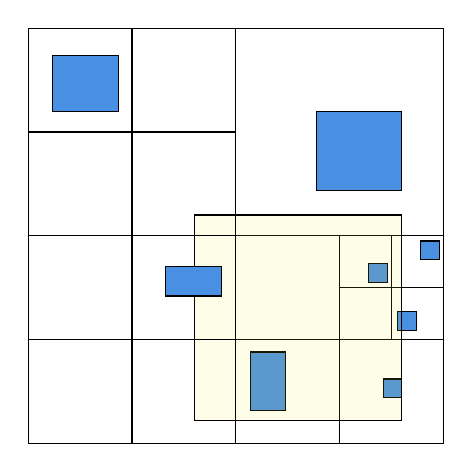
\begin{tikzpicture}[x=0.75pt,y=0.75pt,yscale=-1,xscale=1]
%uncomment if require: \path (0,300); %set diagram left start at 0, and has height of 300
%Shape: Grid [id:dp37542913168733505] 
\draw  [draw opacity=0] (211,35) -- (411,35) -- (411,235) -- (211,235) -- cycle ; \draw   (311,35) -- (311,235) ; \draw   (211,135) -- (411,135) ; \draw   (211,35) -- (411,35) -- (411,235) -- (211,235) -- cycle ;
%Shape: Grid [id:dp9750791482935114] 
\draw  [draw opacity=0] (311,135) -- (411,135) -- (411,235) -- (311,235) -- cycle ; \draw   (361,135) -- (361,235) ; \draw   (311,185) -- (411,185) ; \draw   (311,135) -- (411,135) -- (411,235) -- (311,235) -- cycle ;
%Shape: Grid [id:dp7892168057908815] 
\draw  [draw opacity=0] (361,135) -- (411,135) -- (411,185) -- (361,185) -- cycle ; \draw   (386,135) -- (386,185) ; \draw   (361,160) -- (411,160) ; \draw   (361,135) -- (411,135) -- (411,185) -- (361,185) -- cycle ;
%Shape: Rectangle [id:dp6060962911152178] 
\draw  [fill={rgb, 255:red, 74; green, 144; blue, 226 }  ,fill opacity=1 ] (318,191) -- (335,191) -- (335,219) -- (318,219) -- cycle ;
%Shape: Square [id:dp5321338766394932] 
\draw  [fill={rgb, 255:red, 74; green, 144; blue, 226 }  ,fill opacity=1 ] (400,137.5) -- (409,137.5) -- (409,146.5) -- (400,146.5) -- cycle ;
%Shape: Rectangle [id:dp15366556085797622] 
\draw  [fill={rgb, 255:red, 74; green, 144; blue, 226 }  ,fill opacity=1 ] (222.5,48.25) -- (254.5,48.25) -- (254.5,75.25) -- (222.5,75.25) -- cycle ;
%Shape: Square [id:dp12763621362581] 
\draw  [fill={rgb, 255:red, 74; green, 144; blue, 226 }  ,fill opacity=1 ] (375,148.5) -- (384,148.5) -- (384,157.5) -- (375,157.5) -- cycle ;
%Shape: Square [id:dp5679476241121324] 
\draw  [fill={rgb, 255:red, 74; green, 144; blue, 226 }  ,fill opacity=1 ] (389,171.5) -- (398,171.5) -- (398,180.5) -- (389,180.5) -- cycle ;
%Shape: Square [id:dp8942121948129986] 
\draw  [fill={rgb, 255:red, 74; green, 144; blue, 226 }  ,fill opacity=1 ] (382,204) -- (391,204) -- (391,213) -- (382,213) -- cycle ;
%Shape: Rectangle [id:dp04023637035985317] 
\draw  [fill={rgb, 255:red, 248; green, 231; blue, 28 }  ,fill opacity=0.1 ] (291,125) -- (391,125) -- (391,224) -- (291,224) -- cycle ;
%Shape: Grid [id:dp5558545847926403] 
\draw  [draw opacity=0] (211,135) -- (311,135) -- (311,235) -- (211,235) -- cycle ; \draw   (261,135) -- (261,235) ; \draw   (211,185) -- (311,185) ; \draw   (211,135) -- (311,135) -- (311,235) -- (211,235) -- cycle ;
%Shape: Grid [id:dp3022965469884248] 
\draw  [draw opacity=0] (211,35) -- (311,35) -- (311,135) -- (211,135) -- cycle ; \draw   (261,35) -- (261,135) ; \draw   (211,85) -- (311,85) ; \draw   (211,35) -- (311,35) -- (311,135) -- (211,135) -- cycle ;
%Shape: Rectangle [id:dp14826936005710334] 
\draw  [fill={rgb, 255:red, 74; green, 144; blue, 226 }  ,fill opacity=1 ] (350,75) -- (391,75) -- (391,113) -- (350,113) -- cycle ;
%Shape: Rectangle [id:dp86948007626014] 
\draw  [fill={rgb, 255:red, 74; green, 144; blue, 226 }  ,fill opacity=1 ] (277,150) -- (304,150) -- (304,164) -- (277,164) -- cycle ;
\end{tikzpicture}
}
\subfigure[OpenVDB实现]{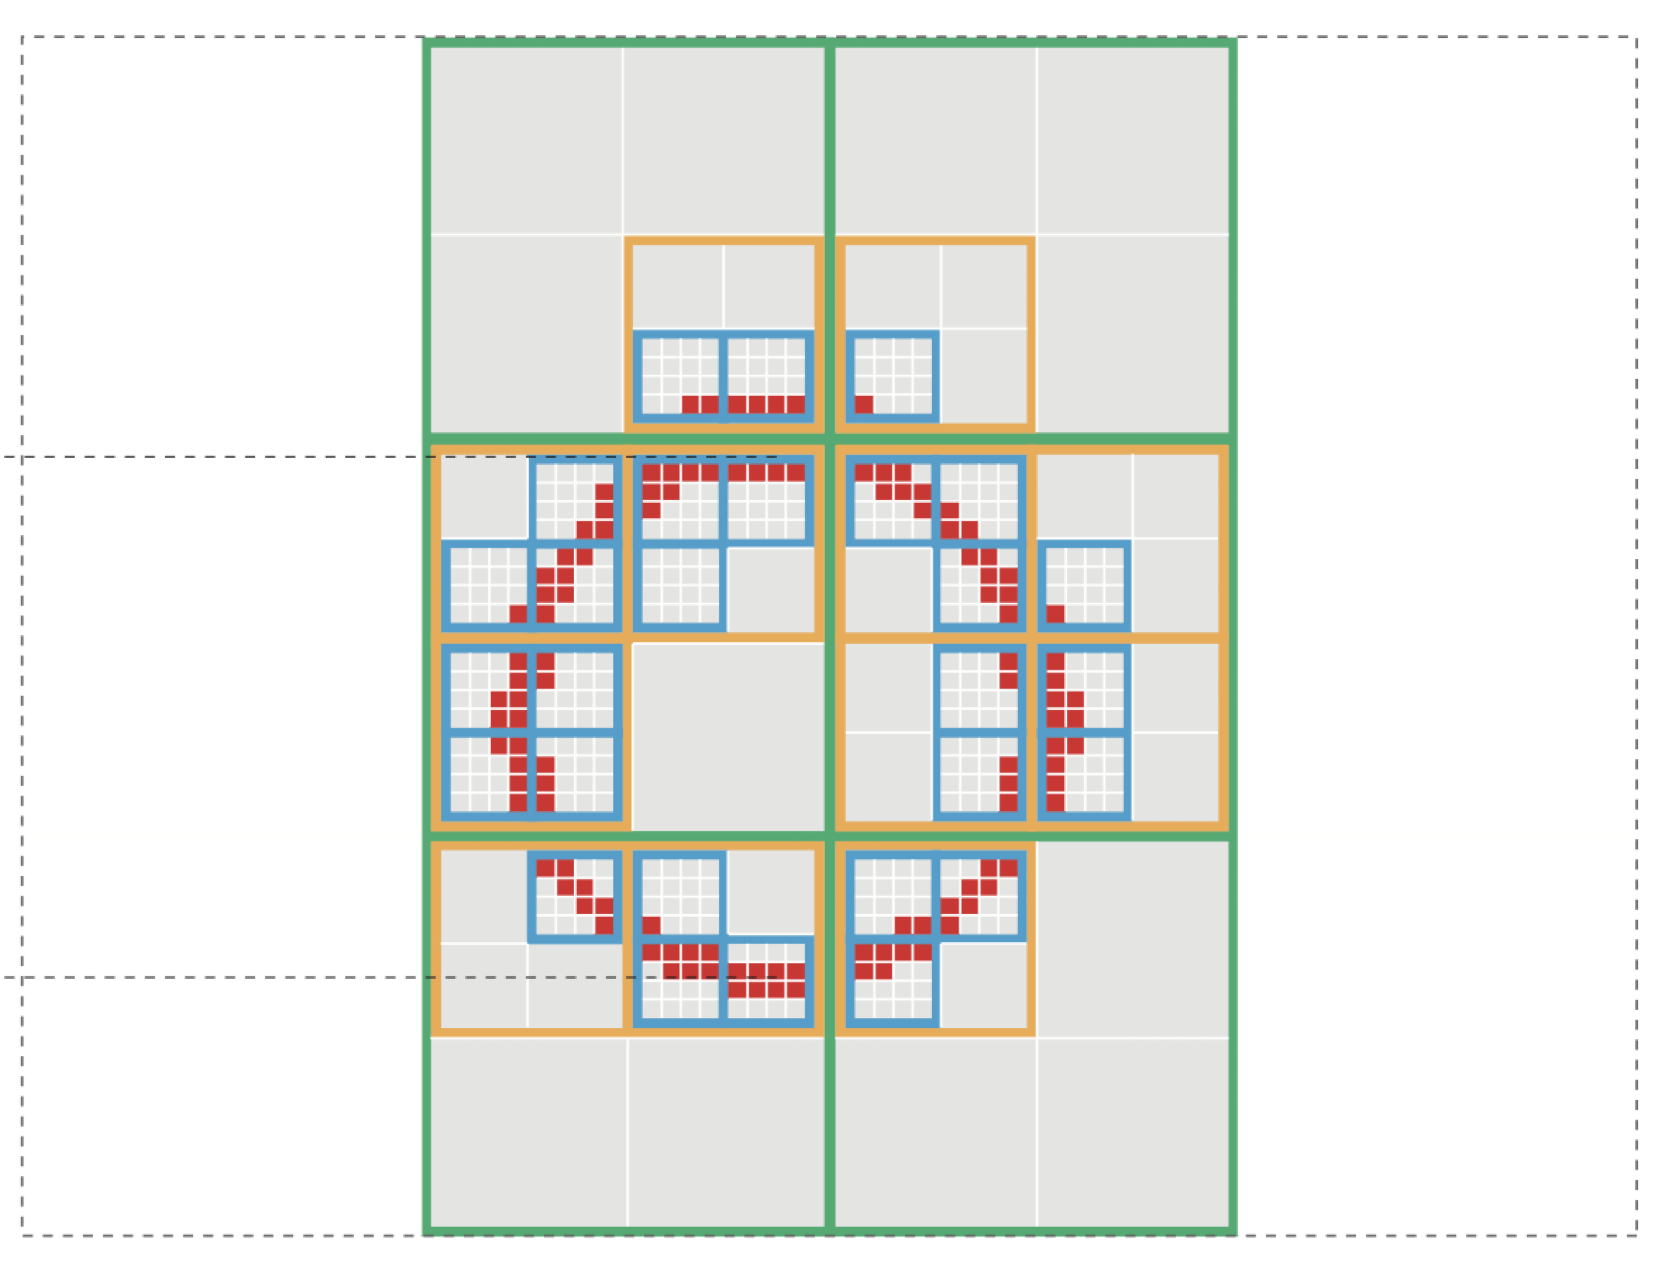
\includegraphics[width=0.425\linewidth]{img/vdb.png}}
  \caption{空间数据结构的实现:左图蓝色表明空间中存在的AABB,黄色部分表明查找范围;右图为OpenVDB对于空间数据的存储方式。}
\end{figure}

构建空间数据结构的速度是碰撞检测的主要性能瓶颈,基于树的空间数据结构的一大问题是其相对难以进行并行。但Sparse Grid能够对已经排序好的一列AABB进行并行的构建,并能有效避免树的层数过高的问题。

Sparse Grid需要指定一个Cell的边长最大值$l$(通常为1),以及最大划分粒度 $k$。每一次进行空间划分都将空间划分为$2^3$份(xyz-轴各二等分),对于每一个边长为$l$的Cell,都至多进行$k$层划分。对于每一个AABB,其都尝试找到最适合的划分块插入。并行构建Sparse Grid的算法如下:

\begin{algorithm}
  \caption{Parallel Sparse Grid Build}\label{alg:ipc-fluid-final}
  \begin{algorithmic}[1]
    \Require 流体粒子包围盒 $\mathbf B$,Sparse Grid参数 $l, k$
    \Ensure Sparse Grid $G$
    \State 确定每一个流体粒子所在Sparse Grid中的位置,并按照边长为$l$的Cell编号排序
    \State 创建所需要的边长为$l$的Cell,并行地将所有排序后的粒子插入
  \end{algorithmic}
\end{algorithm}

在细阶段,本文沿用了基于三次方程的连续碰撞检测模型。记CCD起始点的流体、三角形顶点的位置分别为$\mathbf{f},\mathbf{x}_{1},\mathbf{x}_{2},\mathbf{x}_{3}$,以及更新位置$\mathbf{f}',\mathbf{x}'_{1},\mathbf{x}'_{2},\mathbf{x}'_{3}$其基于以下的方程求解:
\begin{equation}
  \exists t \in [0, 1]\quad \begin{cases}
\det \left[\mathbf x_{1,f} \mathbf x_{2,f}\mathbf x_{3,f}\right] = 0\\
\mathbf x_4 \in \triangle \mathbf x_1\mathbf x_2\mathbf x_3
\end{cases}
\end{equation}
其中$\mathbf x_{i,f} = t (\mathbf x_i ' -\mathbf f') + (1-t) (\mathbf x_i -\mathbf f)$

相对容易求解的是方程中的行列式部分,其是一个关于$t$的三次方程,本文实现的算法基于在区间$[0,1]$内三点进行牛顿迭代,确保不遗漏其在区间内的任一解。该算法能够进行快速求解,并在CCD-Benchmark中获得了其他求解器不拥有的性能优势,如表\ref{tab:ccd-benchmark}所示。

\begin{table}
\centering
\begin{tabular}{l|cccc}
   & IRF & TCCD & TI & 本文\\
  \hline
  t& 115.89 & 0.24 & 0.74 & 0.1 \\
  FP& 2 & 95638 & 2 & 2\\
  FN& 0 & 0 & 0 & 0
\end{tabular}
\caption{CCD-Benchmark结果:本文方法在求解速度、精确度、鲁棒性上都相比以往方法有极大的提升。}\label{tab:ccd-benchmark}
\end{table}

\subsection{ADMM-IPC结果}

基于以上内容,本文实现了ADMM-IPC算法,并在简单场景下进行了测试,下图展示了其流固耦合结果,场景设置为一斜放着的布料,与上方落下的水团进行耦合。

\begin{figure}
  \centering
  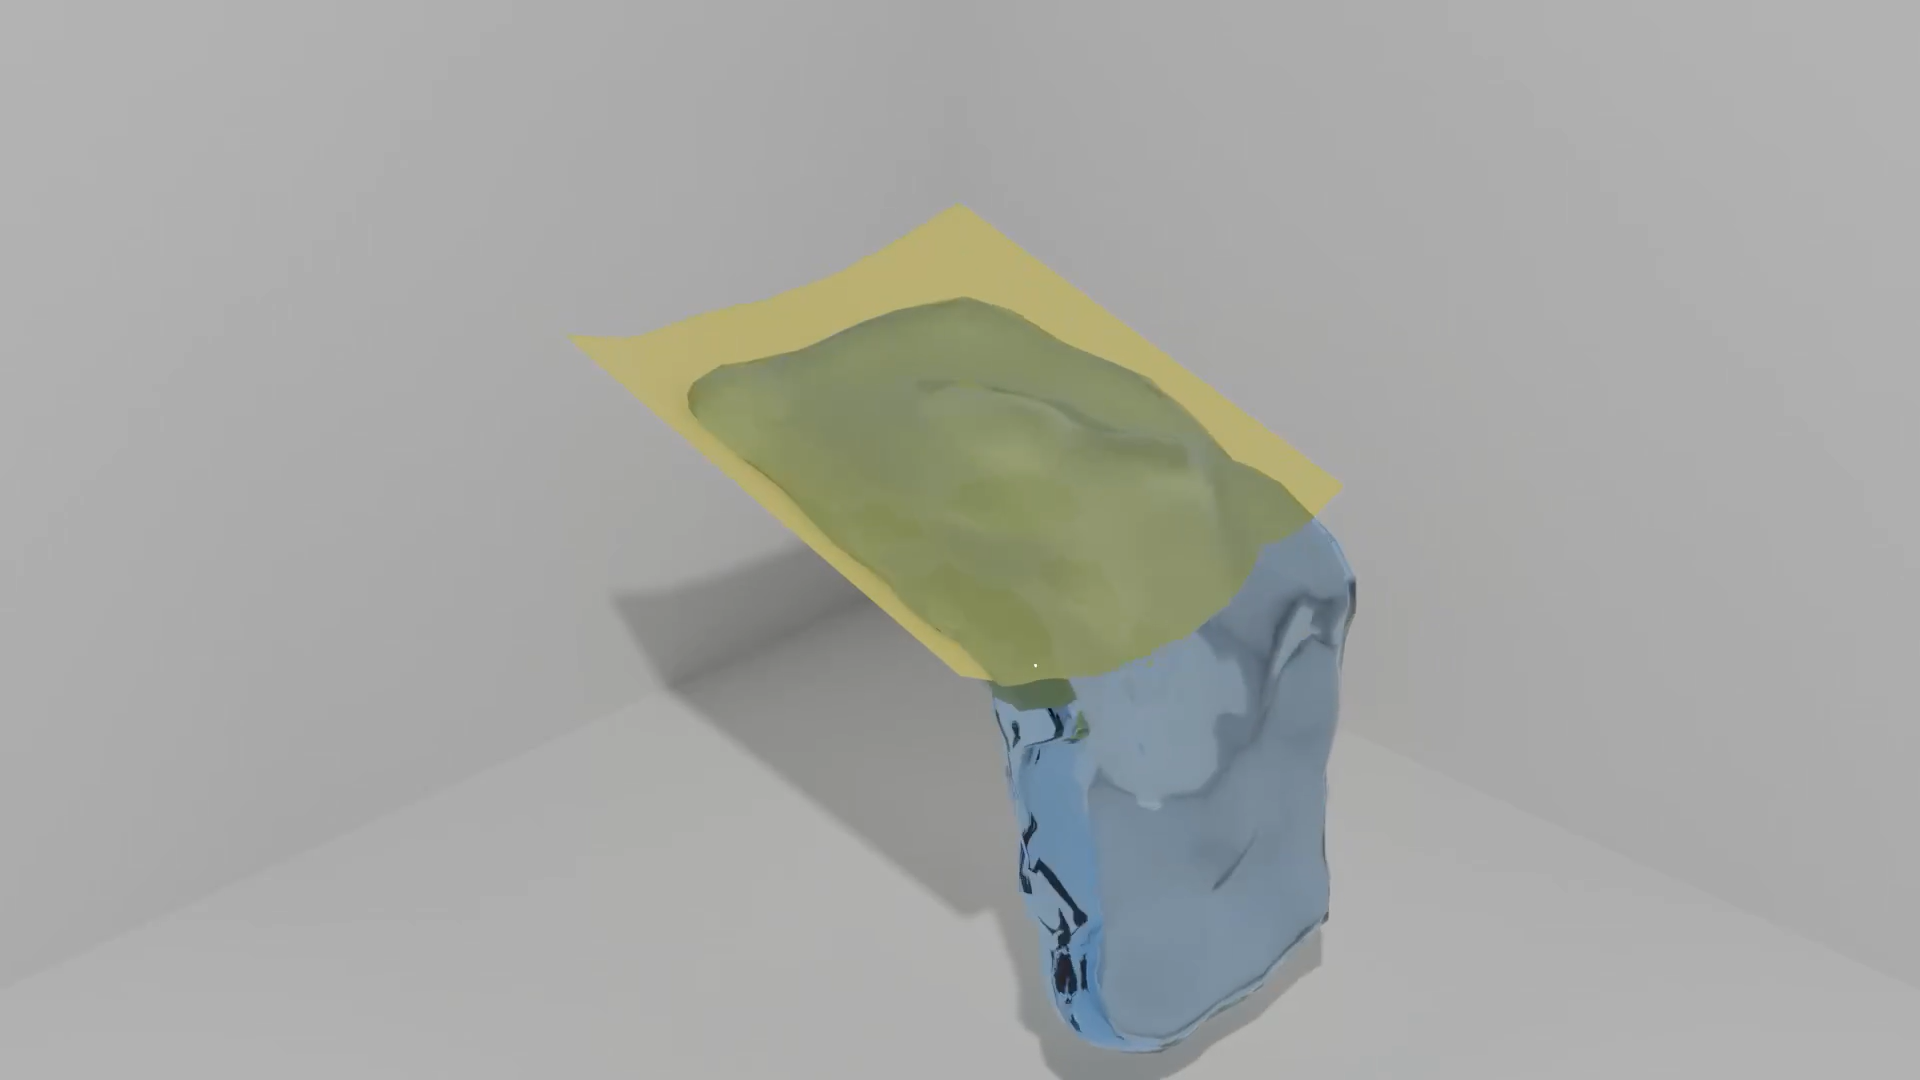
\includegraphics[width=0.9\linewidth]{img/well rendered-0001.png}
\end{figure}

